\documentclass{article}	
\usepackage[a4paper, portrait, margin=1in]{geometry}
\usepackage{amsmath, graphicx, gensymb, float}
\usepackage{chngcntr}
\counterwithin{figure}{section}
\graphicspath{{./images/}}
\usepackage[utf8]{inputenc}
\usepackage{textcomp}
\usepackage[english, macedonian]{babel}
\title{Мехатронички Системи: Управување со Повратна Врска}
\date{16/12/17}
\author{Галевски Марко 1172, Никола Мучев 1017, Елена Наумовска 1019}

\begin{document}
    \pagenumbering{gobble}
    \maketitle{}
    \newpage
    \tableofcontents
    \newpage
    \pagenumbering{arabic}

\section{Вовед}
Роботика и автоматика стануваат потребни и основни делови од инженерството и следствено се многу важни теми за проучување од страна на студенти на инженерство и наука. Понатаму, роботика е изградена врз темели како карактеризација на трансдусери, контрола на мотори, собирање на податоци, механика на движење, мрежна комуникација, компјутерска перцепција, препознавање на шеми, кинематика, планирање на траекторија, и други кои исто така се темели за други полиња како на пример производство. National Instruments (NI) LabVIEW комплетот за роботика заедно со LabVIEW програмскиот пакет нудат додаток на традиционалните учебници за роботика, со можност за активно/практично учење во компактен и проширлив комплет.

%these next 2 paragraphs need to be reworded a bit

Проектот беше изработен со цел да го прикаже концептот и принципот позади управувањето на некој систем со повратна врска. За остварувањето на задачата употребивме еден почетен кит за роботика од National Instruments, роботот DaNI 2.0. Овој роботски кит ги содржи сите компоненти потребни за успешна реализација на задачи и проекти поврзани со управувањето и задвижувањето на еден општ робот во форма на „Rover“. 

Во текот на овој документ ќе се разговара за структурата на роботот - односно неговите сензори и актуатори, како и за управувачката единица sbRIO, исто од NI. Потоа, ќе се претставаат и образложаат 3 алгоритми во LabVIEW. Првите два ќе бидат базирани на ПИД управување со повратна врска, додека третиот алгоритам ќе биде едно детално објаснување на почетната програмата дадена од NI како пример за можните способности на DaNI. За крај, ќе се продискутира за некои предизвици со кои се соочивме во текот на изработката на овој проект, и ќе се разговара за понатамошна работа со DaNI за постигнување на некоја корисна функција.

\begin{figure}[H]
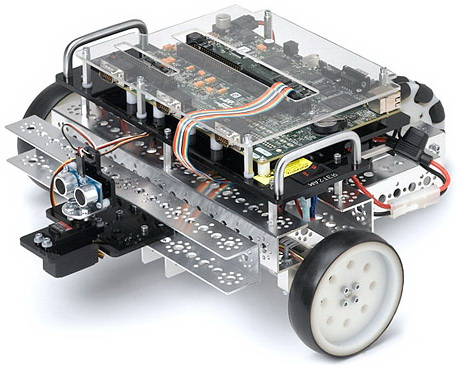
\includegraphics[width=0.75\linewidth]{dani_isometric.jpg}
\centering
\caption{Роботот DaNI}
\label{fig:dani_isometric.jpg}
\end{figure} 

\newpage

\section{DaNI}

National Instruments (NI) LabVIEW комплетот за роботика се состои од DaNI, кој содржи:
\begin{itemize}
	\item Pitsco Education 12 VDC мотори со 152 rpm и 21.6 kg-cm вртежен момент
	\item Оптички квадратурни енкодери со 400 импулси при револуција
	\item PING))) ултразвучен сензор за мерење на растојанја помеѓу 2cm и 3m
	\item PING))) монтажен држач за работен агол од $180 \degree$
	\item Два Pitsco Education TETRIX 10.16cm тркала и едно омни тркало за насочување
	\item sbRIO единица и соодветни кабли за поврзување
\end{itemize}

Хардверот може да биде проучуван, обратно инжениран, и модифициран од студенти. Меѓутоа, главната цел е роботска перцепција и контрола кои се имплементирани во LabVIEW софтвер развиен на одделен сервер (компјутер) и спуштен на роботскиот компјутер.

\begin{figure}[H]
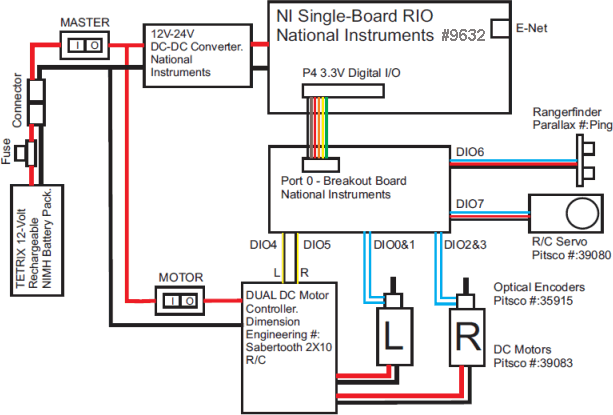
\includegraphics[width=0.75\linewidth]{dani_block_diagram.png}
\centering
\caption{Блок дијаграм на DaNI}
\label{fig:dani_block_diagram.png}
\end{figure}

\subsection{Актуатори}
%NOTE TO SELF: ADD REFERENCES
Од страната на актуатори, DaNI поседува два DC мотори со вградени редуктори, и еден серво мотор. DC моторите се користат за движење на роботот, а серво моторот има улога прецизно да го ротира PING)) ултразвучниот сензор. Подолу се наведени нивните карактеристики.

\subsubsection{DC Мотори}
DC мотор со четкици претставува внатрешно комутиран електричен мотор дизајниран да биде напојуван со извор на еднонасочна струја. Неговата брзина може да се менува со промена на работниот напон или јачината на магнетото поле.
Во DaNI се применети два DC мотори, поточно TETRIX MAX DC мотори.
\renewcommand{\theenumii}{\arabic{enumii}}
\renewcommand{\theenumiii}{\arabic{enumiii}}
\begin{enumerate}
	\item При нормални услови на работа:
	\begin{enumerate}
		\item Номинален напон: $ 6-13.8 V $
		\item Температура на околината: $ -10 \pm 60 \degree C $
		\item Насока на ротација: Спротивно од стрелката на часовникот\\Позитивен пол поврзан со црвен „+“\\Негативен пол поврзан со „-“\\Гледајќи кон оската на излезното вратило		
	\end{enumerate}
	\item Услови на испитување:
	\begin{enumerate}
		\item Напон: DC 12 V
		\item Температура на околината: $ 28 \degree C $
		\item Влажност на воздухот: 44 \% RH
		\item Испитуваниот уред е поставен хоризонтално
	\end{enumerate}
	\item Електрични способности(По 30 секунди напојување)
	\begin{enumerate}
		\item Без оптоварување
		\begin{enumerate}
			\item Брзина: 150 $\pm$ 10 RPM
			\item Струја: 0.34А (0.68А max)
		\end{enumerate}
		\item Со оптоварување
		\begin{enumerate}
			\item Вртежен момент: 3.9kg.cm
			\item Струга: 0.91А (1.37А max)
			\item Брзина: 137.5 $\pm$ 10 \% RPM
			\item Вртежен момент на запирање: /
			\item Струја на запирање: /
		\end{enumerate}
	\end{enumerate}
	\item Механички карактеристики
	\begin{enumerate}
		\item Аксијално поместување на вратилото: $\leq$ 0.5mm
	\end{enumerate}
	\item Својства на моторот:
	\begin{enumerate}
		\item Струја без оптоварување: 0.19А
		\item Брзина без оптоварување: 11000 $\pm$ 10 \% RPM
	\end{enumerate}
\end{enumerate}	

%I think this is some pretty cool stuff and while it doesn't have that much to do with our project in particular I don't really see a reason why it shouldn't be in here considering he asked for 40-50 fucking pages
Двата DC мотори присутни во конструкцијата се контролирани со помош на Sabertooth Dual 10A Motor Driver. Тој може да напојува два DC мотори со четкици со струја до 10А поединечно, со максимални 15А за кратки временски периоди, со многу тивка операција поради ултрасоничната брзина (32kHz) на контрола на неговите транзистори. Sabertooth исто така претставува првиот синхрон регенеративен мотор драјвер во својата класа. Регенеративната топологија значи дека батериите на уредот се полнат кога на уредот му се наредува да забави или да се врати назад, при што исто така ја зголемува и брзината на реакција. Вклучува внатрешно напојување од 5V кое може да напојува микроконтролер или R/C приемник. 

Наредно се зададени техничката скица на моторот со неговите димензии, како и графикот на карактеристики на моторот за различно оптоварување. Овој график ги дава целокупните карактеристики, т.е. карактеристиките на моторот заедно со редукторот.

\begin{figure}[H]
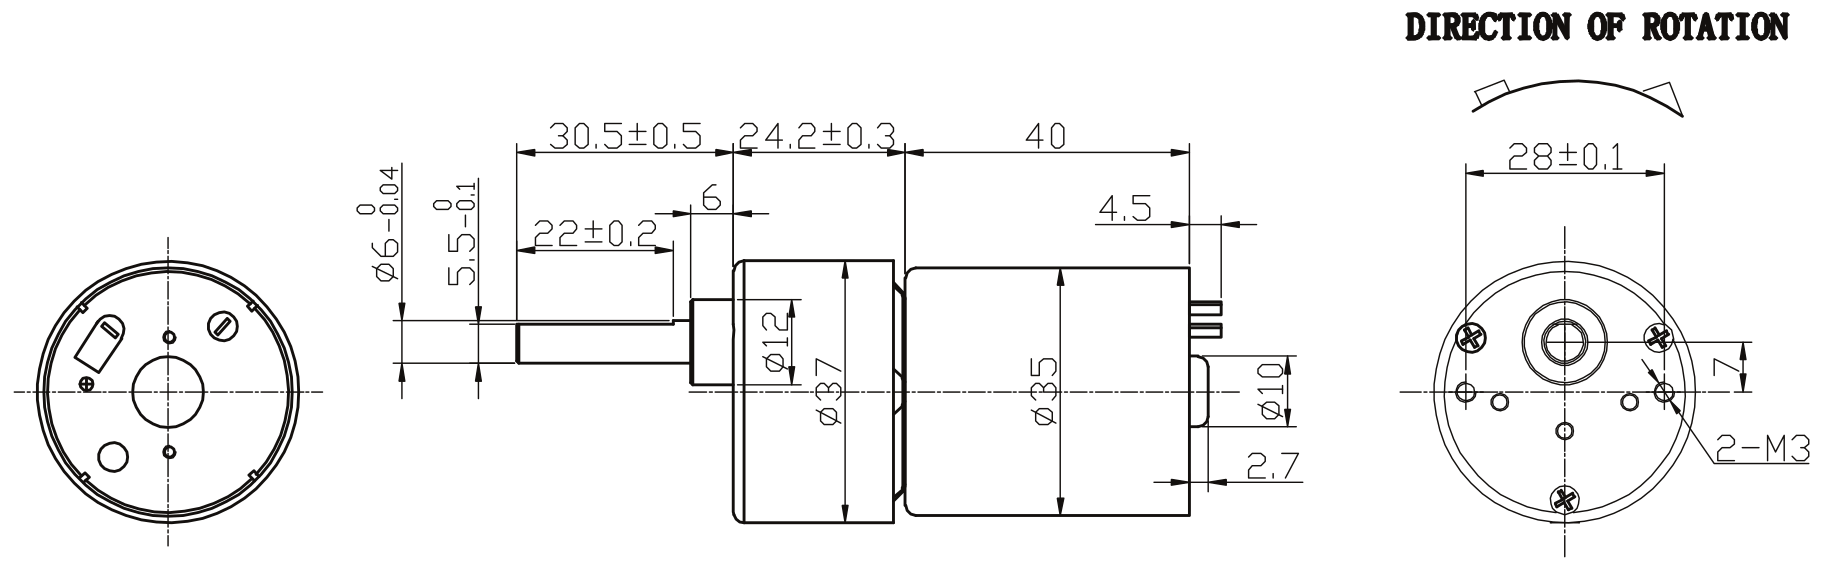
\includegraphics[width=0.75\linewidth]{motor_schematic.png}
\centering
\caption{Техничка скица на DC моторот}
\label{fig:motor_schematic.png}
\end{figure}

\begin{figure}[H]
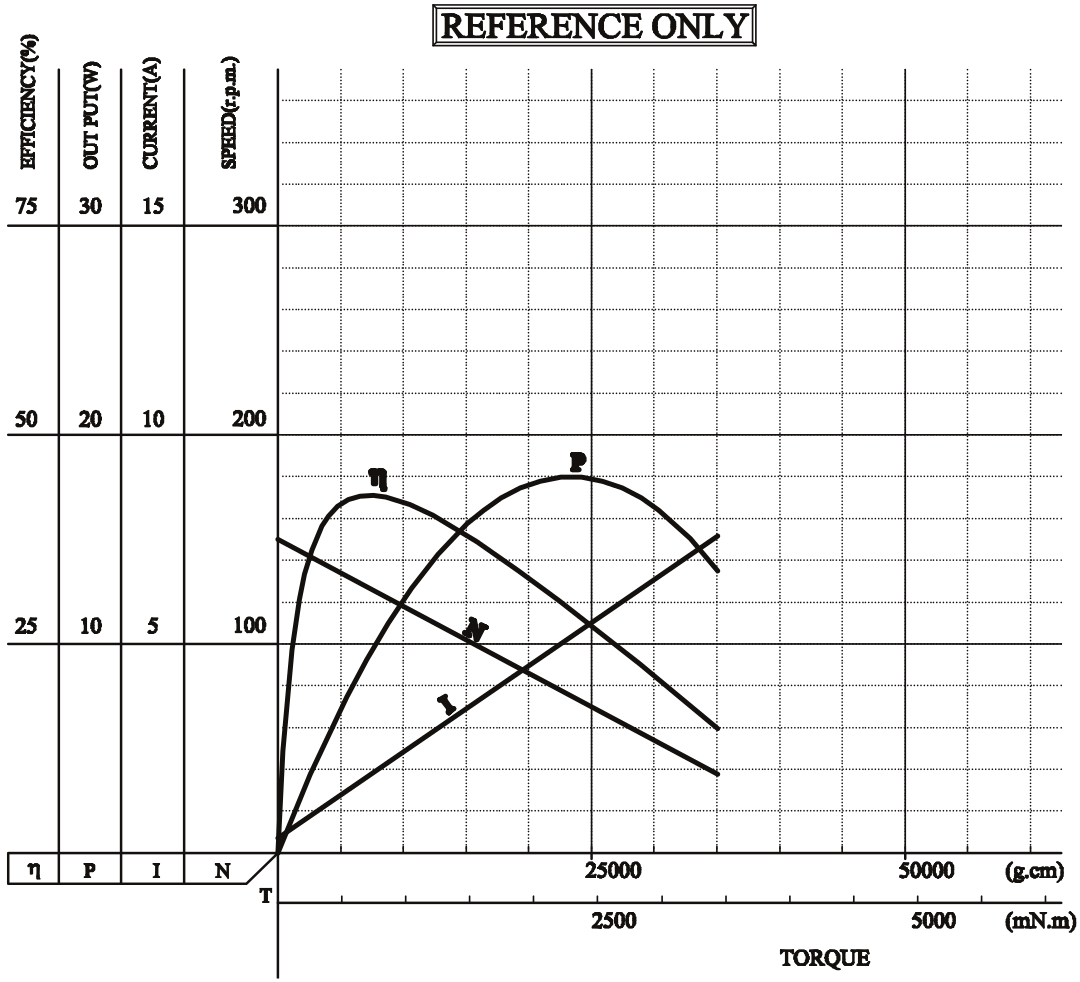
\includegraphics[width=0.75\linewidth]{motor_graph.png}
\centering
\caption{Карактеристични вредности на DC моторот}
\label{fig:motor_graph.png}
\end{figure}

\subsubsection{Серво Мотор}
Серво мотор е ротационен актуатор кој дозволува за прецизна контрола на аголна позиција. Тој се состои од мотор поврзан со сензор за повратни информации за позиција. Исто така има потреба од серво драјвер, кој прима команден сигнал од контролен систем, го засилува сигналот, и пренесува електрична струја до серво моторот со цел да произведе движење пропорционално со командниот сигнал. За оваа цел го користи и сензорот за повратни информации за позиција за да се добие прецизна контрола на ротационата позиција на моторот. Ова е т.н. систем со затворена повратна врска.

Единствена функција на серво моторот во оваа конструкција е ротација на PING)) сензорот, поради што тој не е изложен на значителни оптоварувања.

\begin{table}[h]
\caption{Карактеристики на серво моторот}
\label{tab:title}

\begin{center}
\begin{tabular}{||c|c||}
\hline
Димензии & 39.88 х 19.81 х 37.85mm\\
\hline
Тежина & 45g\\
\hline 
Ранг на напон & 4.8V - 6.0V\\
\hline
Брзина без оптоварување (4.8V) & 0.22sec/60\degree\\
\hline
Брзина без оптоварување (6.0V) & 0.18sec/60\degree\\
\hline
Вртежен момент на запирање (4.8V) & 4.8kg.cm\\ 
\hline
Вртежен момент на запирање (6.0V) & 6.0kg.cm\\
\hline
Максимален ранг на PWM & 553-2425\micro sec\\
\hline
Поминат агол по \micro sec & .102\degree/\micro sec\\
\hline
Максимален пат & 190.5\degree \\
\hline
Амплитуда на импулс & 3-5V \\
\hline
Работна температура & -20\degree C до +60\degree C \\
\hline
Потрошувачка на струја - неактивен (4.8V) & 8mA \\
\hline
Потрошувачка на струја - неактивен (6V) & 8.8mA \\
\hline
Потрошувачка на струја - без оптоварување (4.8V) & 150mA \\
\hline
Потрошувачка на струја - без оптоварување (6V) & 180mA \\
\hline
Можност за континуирана ротација & + \\
\hline
Насока со зголемување на PWM сигнал & Во насока на часовата стрелка \\
\hline
Вид на запченици & Запченици со прави заби \\
\hline
Материјал на запченици & Карбонит \\
\hline
\end{tabular}
\end{center}
\end{table}

\begin{figure}[H]
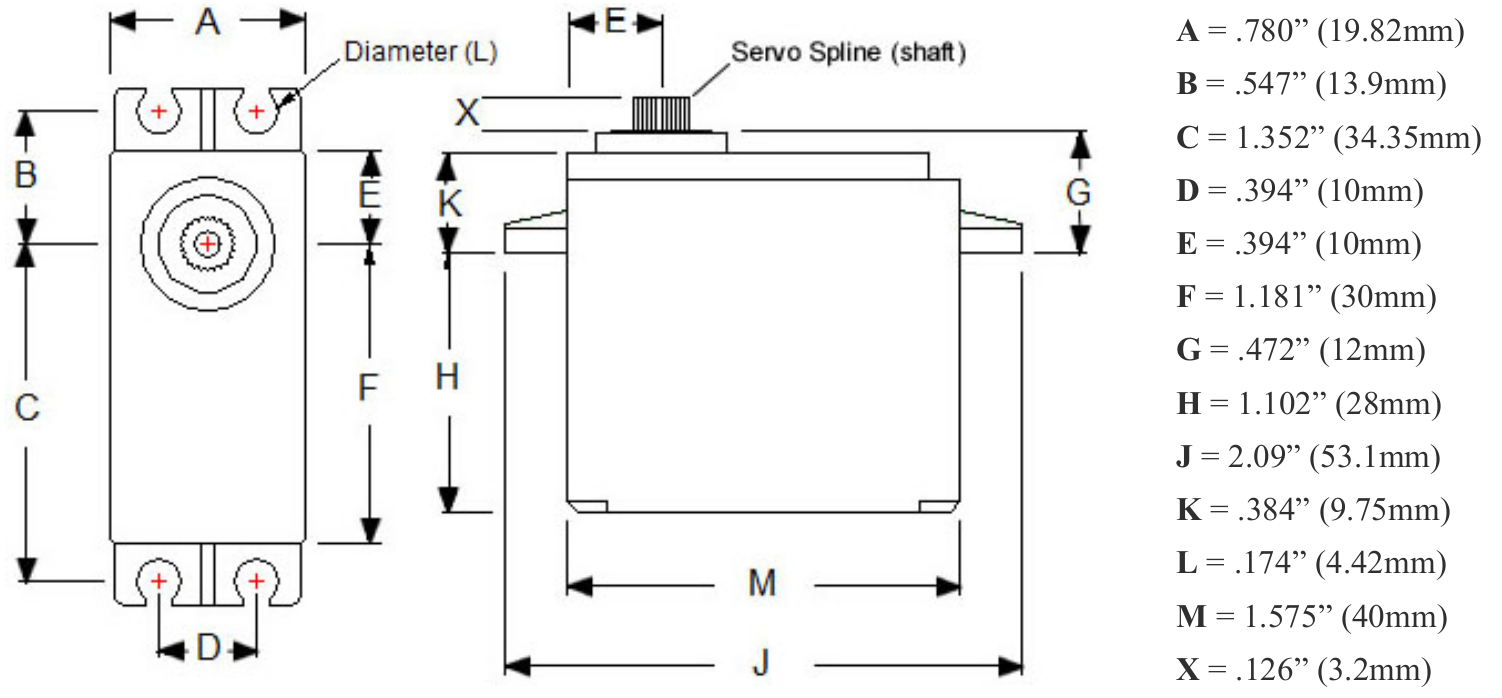
\includegraphics[width=0.75\linewidth]{servo_schematic.png}
\centering
\caption{Техничка скица на серво моторот}
\label{fig:servo_schematic.png}
\end{figure}
\subsubsection{PWM}
PWM (Pulse Width Modulation) е начин на аналогно управување базиран на употребата на чисто дигитални сигнали. При една претходно одредена фреквенција, имаме една соодветна периода, $T(s)$. Во рамките на една периода, можеме да ја дефинираме врската помеѓу времетраењето на активноста (ОN) и времетраењето на неактивноста (OFF) на еден дигитален излез. Добиениот „аналоген“ излез (ефективниот напон) се пресметува со следната равенка:\\
$$ V_{PWM} = V_{dig} \cdot \frac{T_{ON}}{T_{ON} + T_{OFF}} = V_{dig} \cdot \frac{T_{ON}}{T} $$
На пример, ако имаме работна фреквенција 20kHz, имаме периода $50\mu s$. Нека дигиталниот излез биде 5V (т.е. ON = 5V, OFF = 0V). Ако за $30\mu s$ од секоја периода задаваме ON сигнал, а за останатите $20\mu s$ задаваме OFF сигнал, на излез ќе го добиеме ефективен напон:
$$ V_{PWM} = 5 \cdot \frac{30}{30+20} = 5 \cdot 0.6 = 3V $$
\subsection{Сензори}
Во најширока дефиниција, сензор претставува уред, модул или подсистем чија задача е да препознае настани или промени во својата околина, и да испрати согласна информација кон останатата електроника (најчесто компјутерски процесор).

Во DaNI употребуваме два вида на сензори: енкодер и ултразвучен сензор.
\subsubsection{Енкодер}

\begin{figure}[H]
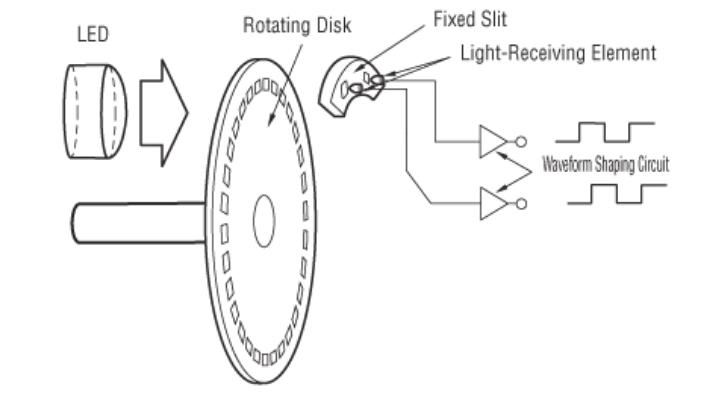
\includegraphics[width=0.75\linewidth]{encoder.png}
\centering
\caption{Шема на оптички енкодер}
\label{fig:encoder.png}
\end{figure}

\subsubsection{Ултразвучен Сензор}
\begin{figure}[H]
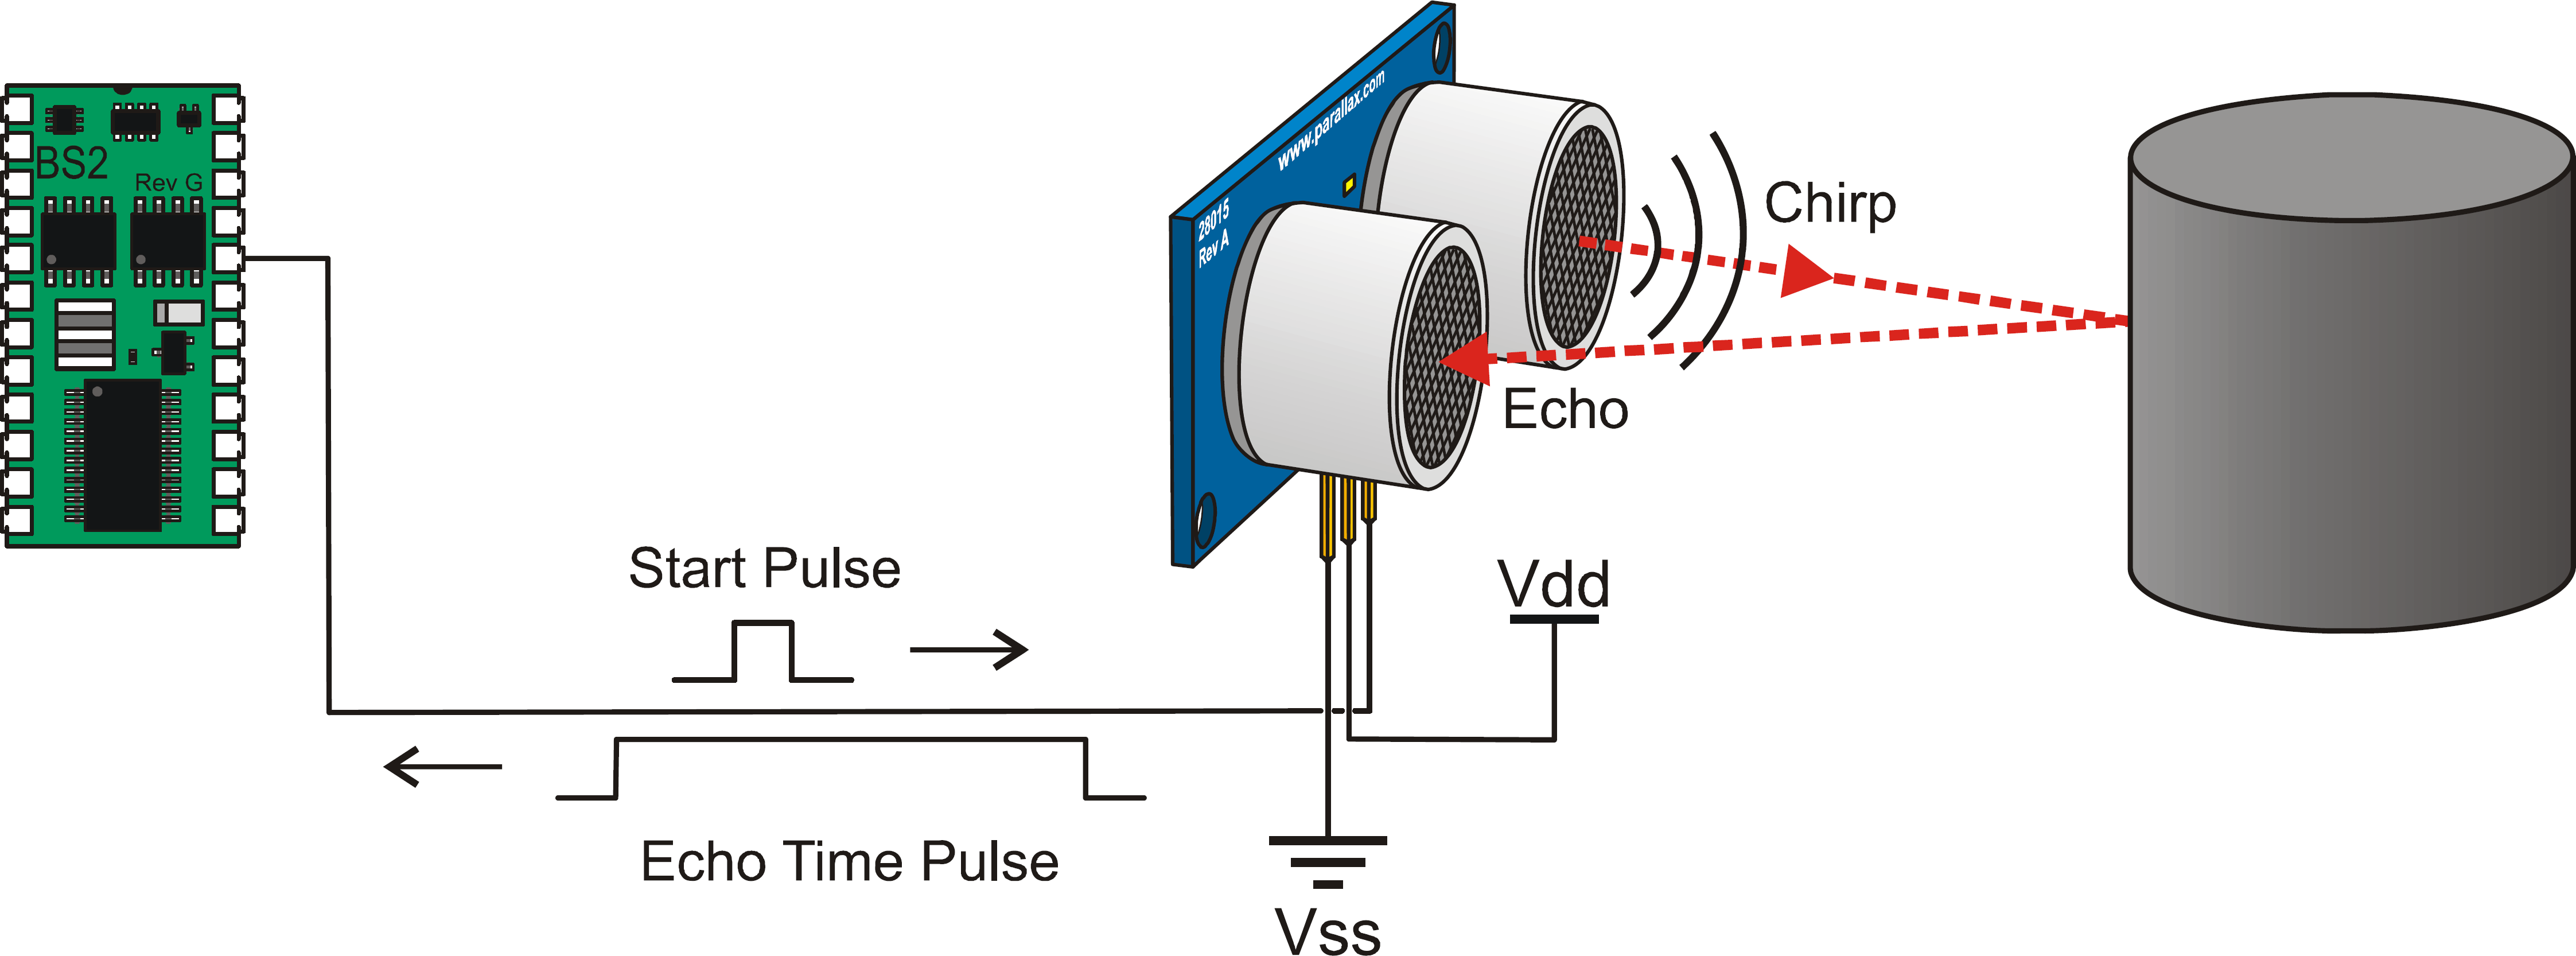
\includegraphics[width=0.75\linewidth]{ping.png}
\centering
\caption{Шема и принцип на дејство на ултразвучен сензор}
\label{fig:ping.ong}
\end{figure}

\newpage
\section{NI sbRIO 9632}

\begin{figure}[h]
\centering
\includegraphics[width=0.75\linewidth]{sb_rio_1.png}
\caption{sbRIO со обележани компоненти}
\label{fig:sb_rio_1.png}

\end{figure}

sbRIO (single-board Reconfigurable Input/Output) управувачките единици од National Instruments претставуваат компјутер монитран на една плочка (single board) наменета за случаи каде што е потребно решение со управување во реално време (Real Time). Оперативен систем кој работи во реално време (RTOS: Real Time Operating System) е изработен со особената цел да извршува функции кои барат големо ниво на временска прецизност и висок степен на надежност. За некој систем да се смета за RTOS, тој мора да има познато максимално време на извршување за секоја од неговите клучни операции. Системите кои можат сигурно да обезбедат максимален временски одѕив се вели дека работаат во потполно реално време, додека системите кои можат само понекогаш да обезбедат максимален временски одѕив се вели дека работаат во делумно реално време.  
 
Потребната брзина се постигнува со истовремето користење на FPGA чип и една обична линеарна процесорска единица. 

sbRIO поседува 110 дигитални влезови/излези, 100 од кои се оспособени за PWM (Pulse Width Modulation), а 10 од кои се наменети за ниско-фреквентна намена. sbRIO поседува и 32 аналогни влезови, и 4 аналогни излези со ранг на излез од $ \pm 10\ V$ со $0.1\%$ грешка при типична употреба на $25\degree C \pm5\degree C$.

sbRIO содржи и 3 сериски „С“ портови за поврзувањето на надворешни модули од NI за проширување на можностите на sbRIO да опфатат и актуација и аквизиција на податоци.

\subsection{FPGA}
FPGA, или „Field Programmable Gate Array“, претставува репрограмибилно интегрално коло кој поседува голем број на програмибилни логични порти. Кај обичните микроконтролери, логиката за управување се пишува и компајлира од некои програмски јазик како C, BASIC или некој графички јазик како G (LabVIEW). Во текот на овој процес се сублимираат во процесорски наредби како ADD и MOV. Низата на можните наредби е единствена за секој микропроцесор. Кај FPGA колата, програмата не се сублимира на наредби, туку самата внатрешна архитектура на колото се подредува со електромагнетни полиња. Како резултат, се добива конфигурација на логични порти која ќе ја извршува задачата опишана во првобитната програма. Бидејќи FPGA нудат хардверско решение, нивното работење е често многу пати побрзо од работењето на обичните микроконтролери, но се подраги.  

\begin{figure}[h]
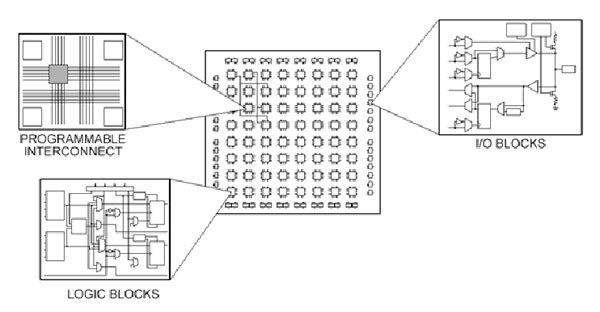
\includegraphics[width=0.75\linewidth]{fpga_diagram.jpg}
\centering
\caption{Приказ на често сретнати термини кај FPGA кола}
\label{fig:fpga_diagram_jpg}
\end{figure}

FPGA колото што се наоѓа во sbRIO-то е моделот Xilinx Spartan 6, кој поседува 6 милиони репрограмибилни логични порти.
\subsection{Споредба со Ардуино Уно}
Ардуино претставува често применето open-source решение за управувачки задачи и во индустрија и на аматерскиот терен. Ардуино плочи често содржат микроконтролер, аналогни-дигитални и дигитални-аналогни претворувачи, и осцилаторски кристал. Додека sbRIO плочите се програмираат во LabVIEW, Ардуино плочите се програмираат во сопствениот „Ардуино“ јазик, која е проширена и поедноставена варијанта на C++ јазикот. Ардуина се популарни помеѓу хобисти, студенти, и за прототипување. Најпопуларната варијанта на Ардуино плочите е Ардуино Уно, која е споредена со sbRIO-то подолу:    
\begin{table}[h]
\caption{Споредба помеѓу Arduino Uno и sbRIO}
\label{tab:title}

\begin{center}
\begin{tabular}{||c|c|c||}
\hline
  & Arduino Uno & NI sbRIO 9632 \\ [0.75ex]
\hline \hline
Напојување & 7 - 12 V DC & 19 - 30 V DC \\
\hline 
Дигитален I/O & 14 влезови/излези & 110 влезови/излези \\
\hline
Брзина & 16MHz & 400MHz \\

\hline
Аналогни влезови & 6 влезови & 32 single-ended влезови \\
\hline
Аналогни излези & 6 дигитални пинови способни за PWM & 4 16-bit излези, 100 PWM пинови \\
\hline
Меморија & 2kB RAM, 32kB неволатилна & 128MB RAM, 256MB неволатилна \\ 
\hline
Цена & €15 & €1560 \\ [0.5ex]
\hline
\end{tabular}
\end{center}
\end{table}
\newpage
\section{LabVIEW}
LabVIEW (Laboratory Virtual Instrument Engineering Workbench) е софтверски пакет наменет за програмирањето на виртуелни уреди (инструменти) за мониторинг и управување на физички уреди. Инструментите што се програмираат во LabVIEW можат да се компајлираат и да се издават како комплетно независни програми кои можат да се монтираат како главен управувен софтвер на мехатроничките уреди и машини.  LabVIEW инструментите се програмираат користејќи го нивниот сопствен графички програмски јазик, „G“. Да се спомени дека јазикот G и G-Code немат никаква поврзаност меѓу себе.
Основниот пакет на LabVIEW поседува многу од стандардните можности што се очекуваат од било кој програмерски јазик, како што се логички/булови операции, математички операции, и пристап до алатки за визуелизација на податоци. 
LabVIEW може да се прошири (и во некои случаи мора да се прошири) со додатни пакети. На пример, овие пакети можат да содржат готови под-инструменти (sub-VIs) за обработка на сигнали (Signal Processing ), или да овозможуваат соработка помеѓу LabVIEW и некои други технологии (FPGA module). Од овие пакети ние ги употребуваме Real Time, FPGA, и Robotics пакетите. Првите два пакети ни го оспособуваат LabVIEW да програмира FPGA чипови и да управува во реално време, додека Robotics пакетот содржи во себе голем број на готови инструменти за обична и инверзна кинематика, отчитување од сензори, и праќање наредби на моторите. 
Robotics пакетот исто поседува едно подмножество на инструменти наменети само за DaNI 2.0, и со тие го управувавме DaNI роботот.  
\subsection{Robotics Модул: Starter Kit 2.0}
Во Robotics модулот на LabVIEW, од интерес ни се готовите VIs за Starter Kit 2.0, кои содржат во нив потпрограми за иницијализација и деиницијализација на роботот, отчитување од сензорите, и задавање на брзина на ротација на моторите. Тука ќе се набројат и објаснат овие блокови.
\paragraph{Иницијализација:\\}

\begin{figure}[h]
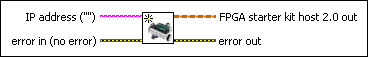
\includegraphics[width=0.45\linewidth]{init.png} 
\raggedright
\caption{VI за иницијализација}
\label{fig:init.png}
\end{figure}

Првиот блок служи за иницијализацита на роботот. Како влез се доведува IP адресата на DaNI роботот, и според зададената адреса започнува комуникацијата со DaNI. При иницијализација на DaNI се создава „објект“ кој го претставува роботот. Програмерскиот термин „објект“ дефинира конгломерат на податоци и функции коj го опишува некој апстрактен предмет. Овие предмети се често неопипливи, но во случаи како нашиот, овој „објект“ е еден кибернетски претставнички меѓуслој кој ни овозможува комуникација со физичкиот систем во прашање. Како излез на оваа функција го добиваме објектот на DaNI, што ни претставува предуслов за употребата на било која од другите фунцкии. Error-in и error-out портите на VI-то се за заштита при некоја грешка во системот. Ако грешката е 1 (има грешка), целата функцијата на иницијализација се заменува со куса врска, и нема излезен објект. \\

\paragraph{Деиницијализација:\\}
\begin{figure}[h]  
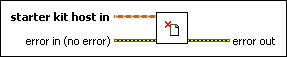
\includegraphics[width = 0.45\linewidth]{deinit.png}
\raggedright
\caption{VI за деиницијализација}
\label{fig:deinit.png}
\end{figure}
Овој блок се става на крај на програма за да се избрише објектот создаден од иницијализацијата, и да се направи соодветен излез. Без оваа крајна фунцкија, грешки се појавуваат при рестартирање на роботот и промени на програмата. 
\\

\paragraph{Управување на моторите:\\}
\begin{figure}[h]
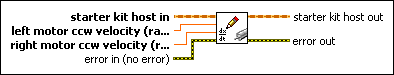
\includegraphics[width=0.45\linewidth]{write_dc.png}
\raggedright
\caption{VI за дефинирање на брзина}
\label{fig:write_dc.png}
\end{figure}

Овој блок е должен за управувањето на брзината на двата DC мотори на DaNI. За функционирањето на блокот потребен е самиот објект на DaNI, како и две вредности за врзините на моторите во \textit{rad/s}. За движење во било која насока, важно е да се опомени дека брзините на моторите морат да бидат со обратен предзнак порадни ниваната обратна поставеност. Моторите имаат максимална брзина на 15.7 \textit{rad/s}.

\paragraph{Отчитување од енкодерите:\\}
\begin{figure}[h]
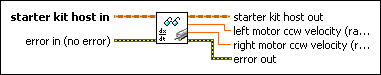
\includegraphics[width=0.45\linewidth]{read_dc.png}
\raggedright
\caption{VI за отчитување од енкодерите}
\label{fig:read_dc.png}
\end{figure}

Со овој блок се отчитуваат моменталните вредности од енкодерите на двата мотори на DaNI. Излезните вредности се во \textit{rad/s} и  имаат \textit{float} формат, и заради тоа можат директно да се прикажат на \textit{display}, во \textit{chart} да се претставаат, или да се вклучат во други пресметки или контролери.

\paragraph{Отчитување од ултразвучниот сензор:\\}
\begin{figure}[H]
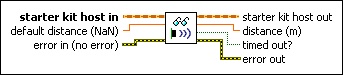
\includegraphics[width=0.45\linewidth]{read_ping.png}
\raggedright
\caption{VI за отчитување од ултразвучниот сензор}
\label{fig:read_ping.png}
\end{figure}

Овој блок служи за отчитување на информацијата дадена од ултразвучниот сензор, монтиран врз серво мотор на предниот дел од DaNI. Отчитаните вредности се исто во формат \textit{float} и се во мерна единица метри.

\paragraph{Насочување на ултразвучниот сензор:\\}
\begin{figure}[H]
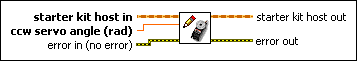
\includegraphics[width=0.45\linewidth]{write_servo.png}
\caption{VI за насочување на ултразвучниот сензор}
\label{fig:write_servo.png}
\raggedright
\end{figure}  
Со овој блок се управува серво моторот на DaNI, односно се одредува поставеноста на ултразвучниот сензор. Блокот како влезови ги прима објектот на DaNI и посаканиот агол во радијани. Право пред роботот се смета за 0, позитивни вредности го вртат сензорот на лево, додека негативни вредности го вртат сензорот на десно. Доменот на сензорот е $ \pm \frac{\pi}{2}$, или $\pm 90 \degree$.

\newpage
\section{Управување со повратна врска}
\subsection{ПИД контролери}
\subsubsection{ПИД контролери во LabVIEW}
За ЕЛЕНА:
Гледај во кодот да ги видиш примерите за како се пишат равенки.

\paragraph{Пример со наброени равенки:}
\begin{equation}
	a = b^2 + \sqrt{\frac{7 \cdot x}{{\ddot x + 3 \cdot \dot x + \int_a^b{x dt}}}}
\end{equation}


\paragraph{Пример со нова линија:}

$$ a = b^2 + \sqrt{\frac{7 \cdot x}{{\ddot x + 3 \cdot \dot x + \int_a^b{x dt}}}} $$



\paragraph{Пример со left alignment:}
\begin{flushleft}
$ a = b^2 + \sqrt{\frac{7 \cdot x}{{\ddot x + 3 \cdot \dot x + \int_a^b{x dt}}}} $
\end{flushleft}

Исто, равенки можат inline да се пишат вака $\int_{birth}^{death}{struggle dt} = life $.

Good Luck, have fun.
\newpage
\section{Изработени Алгоритми}
Во текот на нашата работа со DaNI роботот, развивме 2 алгоритми за неговото управување. Првиот алгоритам ја имаше задачата да го држи роботот на фиксно растојание од пречката (што се детектираше со ултразвучниот сензор), додека вториот алгоритам беше изработен со цел да се изедначат брзините на двете тркала, бидејќи не се совпаѓае. Двата алгоритми се базираат на управување со повратна врска, употребувајќи ПД контролери. Третиот алгоритам е примерниот алгоритам за избегавање на пречки даден од NI за демонстрација. 

\subsection{Одржување на фиксно растојание со ПД контролер}
%Just a text based description of what's happening on the printout of the program, given by nikola. 
%Start at sensor feedback loop. Explain signal processing and clipping/tolerances. Runs into PID.
%Feed speed into motors, ezpz. 
Овој алгоритам ја има задачата да го одржи роботот на фиксно растојание од некоја детектирана пречка. Ова го постигнува со помош на ултразвучниот сензор на DaNI, VI-та дадени од NI Robotics модулот, и еден од вградените ПИД контролери во LabVIEW.\\ Алгоритамот ќе биде постепено образложен во продолжение:

\begin{enumerate}
\item Започнувајќи од левата страна, првин се повикува блокот за инцијализација (сл.\ref{fig:init.png}). На влез се доведува IP адресата на роботот, кој служи за идентификација на истиот. Како излез на овој блок се добива „објектот“ што го претставува DaNI, и секој од блоковите кој има било какво заемнодејство со роботот мора да прима копија од овој објект.
\item Се повикува блокот за насочување на сензорот (сл.\ref{fig:write_servo.png}) да осигури дека ултразвучниот сензор е насочен токму право пред роботот.
\item Следно алгоритамот влегува во \textit{while} циклус. Во овој \textit{while} циклус се отчитува растојанието од сензорот до пречката со \textit{Read Ping)))} блокот (сл.\ref{fig:read_ping.png}).
\item Ова отчитано растојани се заокружува во нашиот VI - \textit{dp.vi}, кој како влез го прима бројот што се заокружува и бројот на посакани децимални места.
\item Овој заокружен број се доведува до влезот на ПИД контролерот како управувана вредност (process variable). Забелешка: Во нашиот случај И терминот на ПИД-от не се употребува, односно работиме со ПД управување.
\item На блезовите на ПИД-от за пропорционално засилување и диференцијално засилување се доведуваат експериментално одредените константи
\item Излезната вредност од ПИД контролерот се зема како да е брзина во $m/s$, и се употребува за управување на моторите. Се заокружува на сличен начин употреубајќи го \textit{dp.vi}.
\item Заокружената брзина се доведува во влезовите на соодветниот блок (сл.\ref{fig:write_dc.png}). Како што е и претходно наведено, брзината што се доведува до левото тркало мора да се негира.
\item При STOP сигнал, \textit{while} циклусот завршува, и брзината на моторите се подесува на 0.
\item Алгоритамот чека 500ms пред да го повика финалниот блок за деиницијализација (сл.\ref{fig:deinit.png}).  
\end{enumerate}


\begin{figure}[H]
\centering
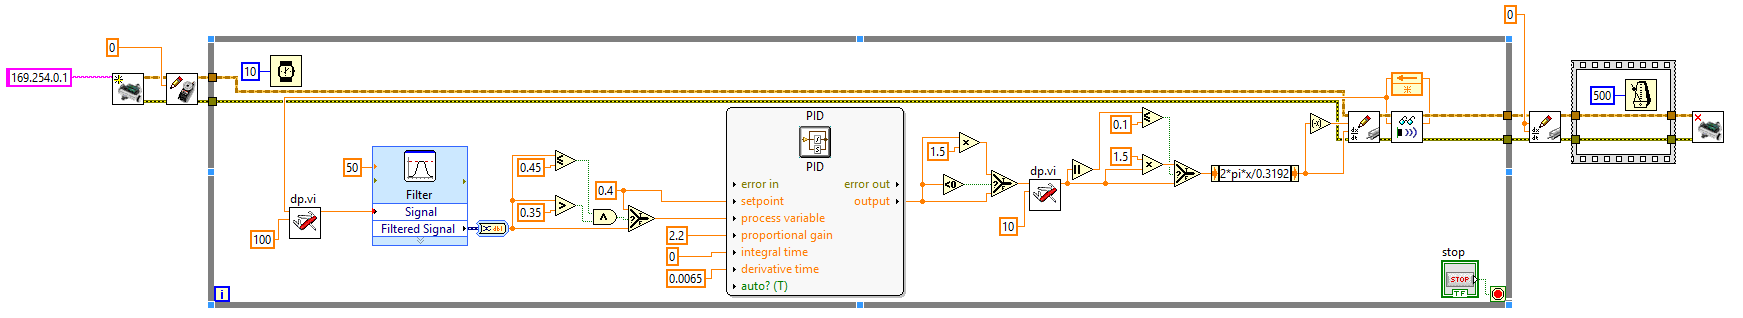
\includegraphics[width = 0.80\paperheight,angle=90]{PID_Control.png}
\caption{Алгоритамот за одржување на растојание}
\label{fig:PID_Control.png}
\end{figure}
\subsection{Компензација на брзинска грешка со ПД контролер}
%Just a proof of concept PID link between left motor and right motor. One will be the setpoint giver, the other will follow and be
%controlled by the PID. Speeds should match up.
%I honestly hope that's what he asked for. To be perfectly honest I don't think he knew exactly what he was asking for either but I've had it up to here (^) with his nonsense, so yeah let's just do this simpler version.
\subsection{Избегавање пречки со хистограм на векторски-полиња}
%OH BOY. This one will be a team effort.
\section{Предизвици}
\section{Заклучок}
\section{Понатамошна работа}
Употребувајќи го тоа што ги имаме научено од проектот, ќе продолжиме од тука да развиеме алгоритам за DaNI што ќе го оспособи прецизно да следи луѓе со помош на фузија на повеќе сензори, како камери и инфра-црвени низи. Можно проширување исто претставува додатокот на уште една камера што ќе може да препознава линии од разни бои, и да ја следи соодветната според изборот на корисникот.
\end{document}

